\documentclass[border=10pt]{standalone}

\usepackage{tikz}
\usepackage{tikzsymbols}
\usetikzlibrary{calc,patterns,shapes.geometric}

\def\centerarc[#1](#2)(#3:#4:#5){\draw[#1] ($(#2)+({#5*cos(#3)},{#5*sin(#3)})$) arc (#3:#4:#5);}

\begin{document}
	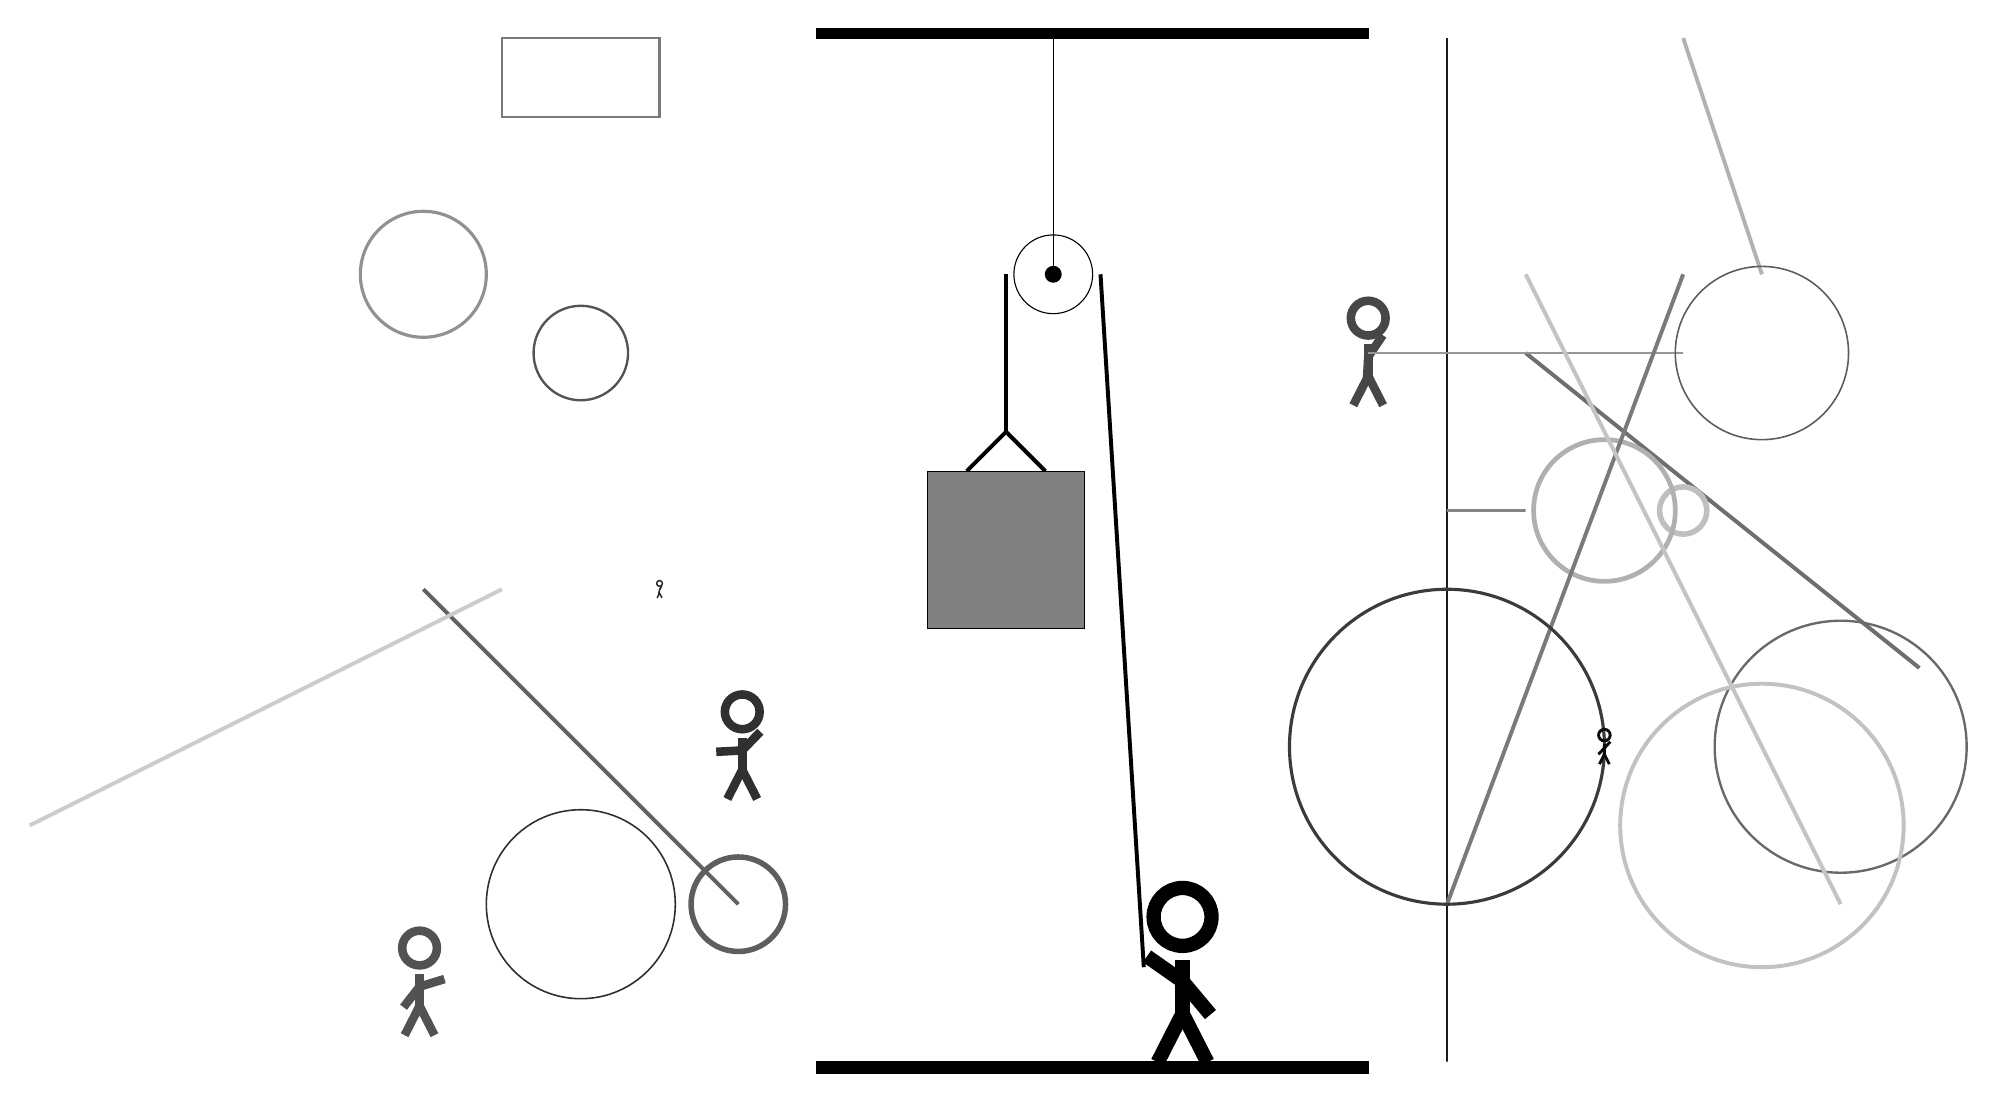
\begin{tikzpicture}
		%%%%% START %%%%%
		
		\draw[fill=black] (-2, 10) rectangle (5, 10.125);
		
		\draw (1, 7) circle (0.5);
		\draw[fill=black] (1, 7) circle (0.1);
		\draw (1, 10) -- (1, 7);
		
		\draw[line width=0.5mm] (-0.1, 4.5) -- (0.4, 5.0) -- (0.9, 4.5);
		\draw[fill=black!50] (-0.6, 4.5) rectangle (1.4, 2.5);
		
		\draw [line width=0.2mm, color=black!82](-5, -1) circle (1.2);
		
		\draw[line width=0.5mm, color=black!57](7, 6) -- (12, 2);
		\draw [line width=0.7mm, color=black!25](9, 4) circle (0.3);
		\draw[line width=0.5mm, color=black!30](9, 10) -- (10, 7);
		\node[line width=0.6mm, color=black!72] at (5, 6) {\Strichmaxerl[6][87][56]};
		
		\draw [line width=0.4mm, color=black!43](-7, 7) circle (0.8);
		\draw[line width=0.5mm, color=black!62](-7, 3) -- (-3, -1);
		\draw [line width=0.6mm, color=black!31](8, 4) circle (0.9);
		\draw [line width=0.3mm, color=black!59](11, 1) circle (1.6);
		\draw[line width=0.3mm, color=black!89] (6, 10) rectangle (6, -3);
		\draw[line width=0.3mm, color=black!41] (5, 6) rectangle (9, 6);
		
		\draw[line width=0.5mm, color=black!52](9, 7) -- (6, -1);
		\draw [line width=0.2mm, color=black!64](10, 6) circle (1.1);
		\draw [line width=0.5mm, color=black!24](10, 0) circle (1.8);
		\draw [line width=0.7mm, color=black!63](-3, -1) circle (0.6);
		\draw [line width=0.4mm, color=black!77](6, 1) circle (2.0);
		
		\draw[line width=0.5mm, color=black!23](7, 7) -- (11, -1);
		\node[line width=0.2mm, color=black!68] at (-7, -2) {\Strichmaxerl[6][52][17]};
		\node[line width=0.2mm, color=black!86] at (-4, 3) {\Strichmaxerl[1][77][61]};
		\node[line width=0.4mm, color=black!81] at (-3, 1) {\Strichmaxerl[6][3][46]};
		\node[line width=0.3mm, color=black!96] at (8, 1) {\Strichmaxerl[2][47][46]};
		\draw[line width=0.5mm, color=black!20](-6, 3) -- (-12, 0);
		
		\draw[line width=0.3mm, color=black!52] (-4, 9) rectangle (-6, 10);
		\draw [line width=0.3mm, color=black!67](-5, 6) circle (0.6);
		\draw[line width=0.4mm, color=black!48] (6, 4) rectangle (7, 4);
		
		\draw[line width=0.5mm] (0.4, 7) -- (0.4, 5.0);
		\centerarc[line width=0.5mm](1, 7)(0:180:0.6);
		\draw[line width=0.5mm](1.6, 7) -- (2.15, -1.8);
		
		\node at (2.6, -1.9) {\Strichmaxerl[10][-35][-50]};
		
		\draw[fill=black] (-2, -3) rectangle (5, -3.15);
		
		%%%%% END %%%%%
	\end{tikzpicture}
\end{document}